\documentclass[a4paper]{article}
\usepackage{fancyhdr}
\usepackage{amsmath}
\usepackage{xcolor}
\usepackage{graphicx}
\usepackage{latexsym}
\usepackage{amssymb}

%%clickable links
\usepackage{hyperref}
\hypersetup{
    colorlinks=true, %colore les liens
    breaklinks=true, %permet le retour à la ligne dans les liens trop longs
    urlcolor= blue, %couleur des hyperliens
    linkcolor= black, %couleur des liens internes
}
%formatted algorithm:
\usepackage{algpseudocode}
\usepackage{algorithm}

\algblockdefx[Event]{Event}{EndEvent}%
[1][]{\textbf{Upon event :} #1}%
{}

\algblockdefx[Data]{Data}{EndData}%
[1][]{\textbf{Data :}}%
{}


\algblockdefx[Init]{Init}{EndInit}%
[1][]{\textbf{Initialization :}}%
{}


%% New commands
\newcommand{\eqdef}{\;\stackrel{\text{def}}{=}\;}

\begin{document}
\title{Distributed Systems: Programming Assignment}
\author{David Benamine \& Rodolphe Lepigre\\
        MOSIG - Parallel, Distributed and Embedded Systems}
        \date{\today}
        \maketitle

        %%%%%%%%%%%%%%%%%%%%%%%%%%%%%%%%%%%%%%%%%%%%%%%%%%%%%%%%%%%%%%%%%%%%%%%%%%%%%%
        \section*{Introduction}
        % TODO

        %%%%%%%%%%%%%%%%%%%%%%%%%%%%%%%%%%%%%%%%%%%%%%%%%%%%%%%%%%%%%%%%%%%%%%%%%%%%%%
        \section{Simulator architecture}
        % TODO

        %%%%%%%%%%%%%%%%%%%%%%%%%%%%%%%%%%%%%%%%%%%%%%%%%%%%%%%%%%%%%%%%%%%%%%%%%%%%%%
        \section{Two regular total-order broadcast protocols}
        % TODO

        \subsection{First protocol}
        % TODO (good latency)

        \subsection{Second protocol}
        % TODO (good throughput with N senders)

        %%%%%%%%%%%%%%%%%%%%%%%%%%%%%%%%%%%%%%%%%%%%%%%%%%%%%%%%%%%%%%%%%%%%%%%%%%%%%%
        \section{Theoretical analysis}
        % TODO

        \subsection{First protocol}
        % TODO
        \begin{itemize}
            \item Optimized for latency
            \item Bad throughput
            \item Every broadcast go through the same tree
            \item $P_0$ is always the broadcast initiator
            \item $P_0$ is responsible for the order
            \item if $P_i$ want to send a message, he sent it to 0 who do the broadcast
            \item Latency : log(N) + 1 (send to 0)
            \item Throughput : todo
        \end{itemize}
        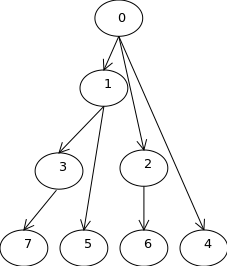
\includegraphics[width=0.5\textwidth]{latencyTO.png}

        \subsubsection{Latency}

        \subsubsection{Throughput}
        % TODO

        \subsection{Second protocol}
        \subsubsection{Principle}
        This protocol is based on the pipeline broadcast protocol but as soon as a node
        receive a message, it will add it to a sorted list. A node $p$ can only deliver the
        first message of its list if this message have been acknowledged by the
        successor of $p$ in the pipeline or if $p$ is the last node of the pipeline.
        This acknowledgement system ensure the total order property (see section
        \ref{sec:pipelineack-proof}).
        \subsubsection{Algorithm}
        \begin{algorithm}[h]
            \centering
                 \begin{algorithmic}
                     \Data
                     \State int : clk
                     \Comment{A logical clock}
                     \State int : next
                     \Comment{the id of the next process in the pipeline}
                     \State int : prec
                     \Comment{the id of the previous process in the pipeline}
                     \State Pending : OrderedList
                     \Comment{A list ordered by clock and id}
                     \EndData
                     \Init
                     \State clk=0
                     \State next=Id()+1\%NProcess
                     \If{Id()==0}
                     \State prec=NProcess
                     \Else
                     \State prec=Id()-1
                     \EndIf
                     \State Pending=EmptyQueue
                     \EndInit
                     \Event $< tob,Broadcast | m> $
                     \State clk++;
                     \State Pending$\rightarrow$add($<m,Id(), clk>$) 
                     \State Send(next,$<m,Id(),clk>$)
                     \EndEvent
                 \end{algorithmic}
            \caption{Pipeline based total ordered broadcast protocol}
        \end{algorithm}
        \begin{itemize}
            \item Optimized for throughput
            \item Aller retour
            \item pipeline
            \item retour sur le pipeline inverse
            \item chaque processus reordonne
            \item delivre si 1 ack recu ET en tete de file
            \item voir TO protocol cours Gruber
            \item trois processus debit 4/3
            \item On acquite la tête de file
        \end{itemize}
        \subsubsection{Proof}
        \label{sec:pipelineack-proof}
        \subsubsection{Latency}
        % TODO

        \subsubsection{Throughput}
        % TODO

        %%%%%%%%%%%%%%%%%%%%%%%%%%%%%%%%%%%%%%%%%%%%%%%%%%%%%%%%%%%%%%%%%%%%%%%%%%%%%%
        \section{Empirical evaluation}
        % TODO

        %%%%%%%%%%%%%%%%%%%%%%%%%%%%%%%%%%%%%%%%%%%%%%%%%%%%%%%%%%%%%%%%%%%%%%%%%%%%%%
        \section*{Conclusion}
        % TODO

        \end{document}

